% !TeX encoding=utf8
% !TeX spellcheck = de_CH_frami

\chapter{BPM auf dem "`Raspberry PI"' in der Domäne "`Home Automation"'}
In diesem Kapitel wird analysiert wie Business Prozesse auf einem Raspberry PI implementiert, beziehungsweise automatisiert werden können. Dabei werden verschiedene Lösungskategorien aufgezeigt und erläutert.


\section{Der Raspberry PI}
\begin{figure}
  \centering
  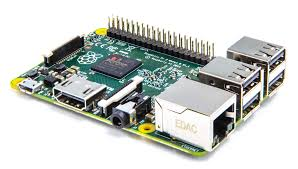
\includegraphics[width=8cm]{./images/RaspberryPi2ModelB}
  \captionsource{Raspberry Pi 2 Model B}{\url{https://www.raspberrypi.org/wp-content/uploads/2015/01/Pi2ModB1GB_-comp.jpeg}}
\end{figure}
  
Der Raspberry Pi ist ein Einplatinencomputer, welcher von der Raspberry Pi Foundation entwickelt und vertrieben wird. Er hat ungefähr die Grösse einer Kreditkarte und bietet zahlreiche On-Board Schnittstellen wie USB-, HDMI und Audio Anschlüsse (Abhängig vom konkreten Modell). Zusätzlich stehen eine bestimmte Anzahl an GPIO-Pins (General Purpose Input / Output) zur Verfügung. Mit Hilfe dieser Pins lassen sich zum einen Erweiterungs-Boards anschliessen und zum anderen können auch über ein spezielles Erweiterungsboard eigene Schaltungen, etc. gebaut und verlötet werden. Die Anzahl und genaue Funktion der einzelnen GPIO-Pins ist vom konkreten Raspberry PI Modell abhängig.

\begin{figure}[H]
  \centering
  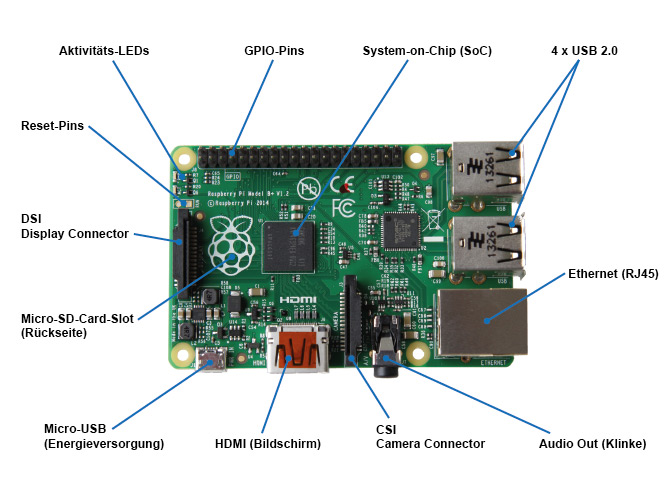
\includegraphics[width=13cm]{./images/RaspberryPi2ModelBPlusOverview}
  \captionsource{Raspberry Pi 2 Model B Überblick}{\url{https://www.elektronik-kompendium.de/sites/raspberry-pi/bilder/19052512.jpg}}
\end{figure}

\newpage
\begin{landscape}

\subsection{Raspberry Pi Modelle im Überblick}
\begin{table}[H]
\centering
\begin{tabular}{r | c  | c | c | c | c | c | c | c | c | c}
	& \THrot{\textbf{Raspberry Pi Model A}}
	& \THrot{\textbf{Raspberry Pi Model A+}}
	& \THrot{\textbf{Raspberry Pi Model B}}
	& \THrot{\textbf{Raspberry Pi Model B+}}
	& \THrot{\textbf{Raspberry Pi 2 Model B}}
	& \THrot{\textbf{Raspberry Pi 3 Model B}}
	& \THrot{\textbf{Raspberry Pi Compute}}
	& \THrot{\textbf{Raspberry Pi Zero}}\\
\midrule
Gewicht in Gramm
	& 	31
	&	23
	&	40		
	& 	45 
	&	40
	&	40
	&	7
	&	9\\
\midrule
System-on-a-Chip (SoC):
	& 	\multicolumn{4}{|c|}{BCM2835} 
	&	BCM2836
	&	BCM2837
	&	\multicolumn{2}{|c|}{BCM2835} \\
\midrule
CPU Kerne
	& 	1
	&	1
	&	1		
	& 	1 
	&	1
	&	4
	&	1
	&	1\\
\midrule
CPU Takt in MHz
	& 	\multicolumn{4}{|c|}{700} 
	&	900
	&	1200
	&	700
	&	1000\\
\midrule
CPU Architektur
	& 	\multicolumn{4}{|c|}{ARMv6 (32-bit)}  
	&	ARMv7 (32-bit)	
	&	ARMv7 (64-bit)	
	&	\multicolumn{2}{|c|}{ARMv6 (32-bit)}  	\\
\midrule
GPU Takt in MHz
	& 	\multicolumn{5}{|c|}{250} 
	&	300/400
	&	\multicolumn{2}{|c|}{250} \\
\midrule
Arbeitsspeicher in MB
	& 	\multicolumn{2}{|c|}{256}  
	&	256 / 512		
	& 	\multicolumn{2}{|c|}{512}  	
	& 	1024 
	&	\multicolumn{2}{|c|}{512}  	\\
	
\midrule
Pins
	& 	26
	&	40
	& 	26
	& 	\multicolumn{3}{|c|}{40}  	
	&	60
	&	40  	\\
	
\midrule
GPIO-Pins
	& 	17	
	&	26
	& 	17
	& 	\multicolumn{3}{|c|}{26}  	
	&	48
	&	26  	\\
\bottomrule
\end{tabular}
\end{table}

%Evtl.: http://praxistipps.chip.de/welcher-raspberry-pi-alle-modelle-im-vergleich_41923

\end{landscape}
\newpage

\section{Betrachteter Lösungsraum}
Ursprünglich wären folgende Einschränkungen für den Lösungsraum vorgesehen gewesen:
\blockquote {Da der Raspberry Pi eine offene Plattform ist, gibt es unterschiedlichste Möglichkeiten um das betrachtete Problem zu lösen. Im Kontext dieser Seminararbeit erfolgt die Betrachtung spezifisch für ein Raspberry Pi 2 Model B mit einem Raspbian OS (Debian Distribution für den Raspberry Pi). Als zusätzliche Prämisse gilt ebenfalls, dass der Kern der Anwendung auf dem Raspberry Pi lauffähig sein muss und die Lösung muss es in irgendeiner Form ermöglichen einen Ablauf / Prozess im Bereich Home Automation mit \gls{acr:BPMN} oder \gls{acr:BPEL} abzubilden. Alternative Lösungen, bei denen der Raspberry Pi als "`Client"' / "`Agent"' verwendet wird sind nicht im Fokus dieser Arbeit.}

Die ersten intensiven Recherchen haben gezeigt, dass es keine bis sehr wenige Lösungen gibt, welche den Grossteil der Anforderungen aus dem Lösungsraum erfüllen würden. Daher habe ich mich entschieden, den Lösungsraum anzupassen und zwei verschiedene Kategorien von Lösungen zu ermöglichen.

\textbf{Spezifische Home Automation Lösungen}
\begin{itemize}
\item Lauffähig auf dem Raspberry Pi mit Raspbian (32-Bit)
\item Eine einzige Komponente (Keine Kombination von Komponenten)
\item Open Source / Frei verfügbar (allenfalls Demoversion)
\item Bedienbar via Web
\item Fokus: Home-Automation
\item Funktionalität um Abläufe oder Aktionen zu automatisieren
\end{itemize}

\textbf{Lösung mit \gls{acr:BPMN}-Support im Bereich \gls{acr:IOT}}
\begin{itemize}
\item Lauffähig auf dem Raspberry Pi mit Raspbian (32-Bit).
\item Eine einzige Komponente (Keine Kombination von Komponenten)
\item Open Source / Frei verfügbar (allenfalls Demoversion)
\item Bedienbar via Web
\item Abläufe / Prozesse können mit Hilfe von \gls{acr:BPMN} modelliert werden.
\item Möglichkeit zur Anbindung von \gls{acr:IOT}-Geräten aus dem Bereich "`Home Automation"' (z.B. via Plugins oder Custom-Code).
\end{itemize}


\section{Lösungen, Produkte \& Frameworks }
In diesem Abschnitt werden die recherchierten Lösungen, Produkte und Frameworks aufgezeigt. Diese Auflistungen sind nicht abschliessend und repräsentieren den Stand der Dinge zum Zeitpunkt der Recherchen im Q2/2016.

\subsection{Lösungskategorie: Spezifische Home Automation Lösungen}
Die Inhalte dieser Lösungskategorie wurden aus dem Kapitel \ref{sec:Analyse:HA:LPF} \nameref{sec:Analyse:HA:LPF} entnommen und nach folgenden Kriterien gefiltert:

\textbf{Filterkriterien}
\begin{itemize}
\item Web-basiert
\item Ready-To-Use
\item Kein Framework
\item Trigger \& Action oder Workflow  / Prozess oder BPMN / BPEL Unterstützung
\item Open Source / frei verfügbar
\item Lauffähig unter Raspbian 32-Bit
\end{itemize}

\textbf{Lösungsraum (gefiltert nach Filterkriterien)}
\begin{itemize}
\item TriggerHappy
\item HomeAssistant
\item openHAB
\item Domogik
\item HomeGenie
\item Freedomotic
\item Domoticz
\end{itemize}

Aufgrund eines kurzen Antestens und des daraus resultierenden Eindruckes wurde "`openHAB"' für die Realisierung des Demo-Setups ausgewählt. Die Auswahl erfolgte nicht aufgrund bestimmter Kriterien. Der genaue Setup wird im Abschnitt \ref{sec:AnalyseRPI:Beispiel} \nameref{sec:AnalyseRPI:Beispiel} beschrieben. Ein Fazit zur ausgewählten Lösung wird im Kapitel \todo{Ref zu Kapitel.}


\subsection{Lösung mit BPMN-Support im Bereich IOT}
Der definierte Lösungsraum dieser Lösungskategorie ermöglicht ein breites Spektrum an Lösungen. Nachfolgend werden einige der möglichen Lösungen aufgezeigt. Bei der Auswahl wurden folgende Kriterien berücksichtigt:

\textbf{Filterkriterien}
\begin{itemize}
\item Web-basiert
\item Ready-To-Use
\item Kein Framework
\item Integrierte \gls{acr:BPMN}-Engine
\item Open Source / frei verfügbar
\item Lauffähig unter Raspbian 32-Bit
\end{itemize}

\textbf{Lösungsraum (gefiltert nach Filterkriterien)}
\begin{itemize}
\item \hyperlink{http://activiti.org/}{activiti BPM Platform}
\item \hyperlink{http://www.jbpm.org/}{jBPM}
\item \hyperlink{https://camunda.com/}{Camunda BPM Platform (Community Edition)}
\item \hyperlink{http://www.imixs.org/}{Imixs Workflow}
\end{itemize}

Aufgrund einer kurzen Analyse, des ersten Eindruckes und der eingeschätzten Komplexität wurde für den Beispielsetup die "`activiti BPM Plattform"' ausgewählt.


%------------------------------------------------------------------
\newpage
\section{Realisierung eines Beispielhaften Prozesses mit BPMN im Bereich "`Home Automation"'} \label{sec:AnalyseRPI:Beispiel}
Nachfolgend wird der realisierte Beispielprozess und die dafür benötigten Komponenten beschrieben.

\subsection{Verwendete Hardware}
Für die Realisierung des Beispiel-Setups wurden folgende Hardware-Komponenten verwendet:
\begin{itemize}
\item \textbf{Raspberry Pi 2 Model B}
\itemBfText{Razberry Board}{Das Razberry Board ist ein Raspberry Pi Erweiterungsboard, welches als Z-Wave Controller eingesetzt werden kann.}
\itemBfText{Z-Wave.Me Double Wall Switch}{Z-Wave Wand-Schalter, welcher mit verschiedenen Funktionen programmiert werden kann.}
\itemBfText{domitech Z-Wave Smart LED Light Bulb}{Z-Wave LED Glühbirne.}
\itemBfText{Ralink Technology, Corp. RT5370 Wireless Adapter}{USB-WLAN Adapter.}
\end{itemize}

\subsection{Verwendete Software}
Für die Realisierung des Beispiel-Setups wurden folgende Software-Komponenten verwendet.
\begin{itemize}
\itemBfText{NOOBS}{\gls{acr:NOOBS} ist ein Hilfsprogramm zur Installation von Betriebssystemen auf dem Raspberry Pi.}

\itemBfText{Raspbian Jessie}{Als Betriebssystem wurde die aktuelle Version von Raspbian Jessie (Debian Derivat).}

\itemBfText{openHAB 2}{Als Schlüsselkomponente wurde openHAB 2 eingesetzt. openHAB 2 ist eine Open Source Lösung für die Heimautomatisierung. Die Basis von openHAB 2 bildet das Eclipse SmartHome Framework der Eclipse Foundation. Die Installation und Konfiguration erfolgte gemäss den Anleitungen und Beispielen im \hyperlink{https://github.com/openhab/openhab/wiki}{GitHub-Wiki von openHAB}.}

\itemBfText{Apache Derby}{Apache Derby ist eine in Java implementierte relationale Datenbank, welche unter der Open Source Apache Lizenz, Version 2.0 verfügbar ist. Die Apache Derby Datenbank wurde verwendet um die Persistenz in openHAB zu realisieren. Die Integration erfolgte über das \gls{acr:JPA} Binding von openHAB. Die Apache Derby Installation wurde gemäss der von Apache zur Verfügung gestellten \hyperlink{https://db.apache.org/derby/papers/DerbyTut/install_software.html}{Anleitung} installiert und konfiguriert. Die Anbindung an openHAB erfolgte gemäss der Dokumentation im \hyperlink{https://github.com/openhab/openhab/wiki/JPA-Persistence}{Wiki}.}

\itemBfText{ejabberd XMPP-Server}{Als \gls{acr:XMPP} Server wurde ejabberd verwendet. \gls{acr:XMPP} Server werden unter anderem für Instant Messaging eingesetzt. In diesem Setup wurde der \gls{acr:XMPP} Server für die Kommunikation zwischen dem openHAB Server und dem Anwender verwendet. Einerseits kann openHAB über ein Binding Nachrichten an den Anwender senden und andererseits kann der Anwender bestimmte Befehle und Anweisungen an openHAB übermittelt. Die Installation von ejabberd erfolgt anhand der Anleitungen von \hyperlink{https://www.digitalocean.com/community/tutorials/how-to-install-ejabberd-xmpp-server-on-ubuntu}{Digitalocean} und \hyperlink{https://box.matto.nl/ejabberdjessie.html}{box.matto.nl}. Das openHAB Binding wurde gemäss der Dokumentationen im openHAB-Wik eingerichtet (\hyperlink{https://github.com/openhab/openhab/wiki/Actions\#xmpp-actions}{Action-Bindings}, \hyperlink{https://github.com/openhab/openhab/wiki/Feature-Overview}{UI's}).}

\itemBfText{Mosquitto MQTT Broker}{Mosquitto ist ein Open Source \gls{acr:MQTT} Broker der Eclipse Foundation. \gls{acr:MQTT} ist ein leichtgewichtiges "`Publish-Subscribe"' Protokoll auf Basis von TCP/IP. Innerhalb von openHAB kann \gls{acr:MQTT} unter anderem für die Publikation des aktuellen Status der Geräte / Komponenten verwendet werden. Ebenfalls können Statusänderungen an Geräten / Komponenten über den \gls{acr:MQTT} Server durchgeführt werden. Mosquitto wurde gemäss der Anleitung von \hyperlink{https://www.digitalocean.com/community/questions/how-to-setup-a-mosquitto-mqtt-server-and-receive-data-from-owntracks}{Digitalocean} installiert. Die Konfiguration in openHAB erfolgte gemäss der Anleitung im \hyperlink{https://github.com/openhab/openhab/wiki/MQTT-Binding}{Wiki}.}

\itemBfText{openHAB Bindings}{Neben den beschriebenen Komponenten wurden diverse weitere Bindings und Actions innerhalb von openHAB verwendet.}

\itemBfText{Apache Tomcat 7}{Um die BPM Plattform "`activiti"' zu nutzen wurde der Open Source Web Server Apache Tomcat 7 eingesetzt. Die Installation erfolgte gemäss der Anleitung von \hyperlink{https://www.digitalocean.com/community/tutorials/how-to-install-apache-tomcat-7-on-ubuntu-14-04-via-apt-get}{Digitalocean}}.

\itemBfText{activiti BPM Plattform}{Activiti ist eine Java-basierte Open Source Workflow und \gls{acr:BPM} Plattform. Die Beispielsapplikation wurde gemäss den Informationen im \hyperlink{http://activiti.org/userguide/index.html}{User-Guide} und den Beispiels-Anwendungen "`activiti-explorer"' und "`activiti-rest"' implementiert. }

\itemBfText{H2}{Die H2 Datenbank ist eine Open Source Java SQL Datenbank, welche als Backend der activiti BPM Plattform eingesetz wird. Die Installation erfolgte gemäss der Anleitung von \hyperlink{http://www.h2database.com/html/tutorial.html}{H2}.}


\itemBfText{Pidgin Internet Messenger}{Auf der Client-Seite wurde für die Kommunikation mit ejabberd der "`Pidgin Internet Messenger"' verwendet.}

\itemBfText{Linux Utilities und Tools}{Es wurden diverse weitere Linus-Utilites und Tools für die Implementation und die Arbeit mit den Komponenten verwendet (unter anderem: screen, scp, Eclipse IDE).}
\end{itemize}

\newpage
\begin{landscape}
\subsection{Komponentenübersicht}
\begin{figure}[H]
  \centering
  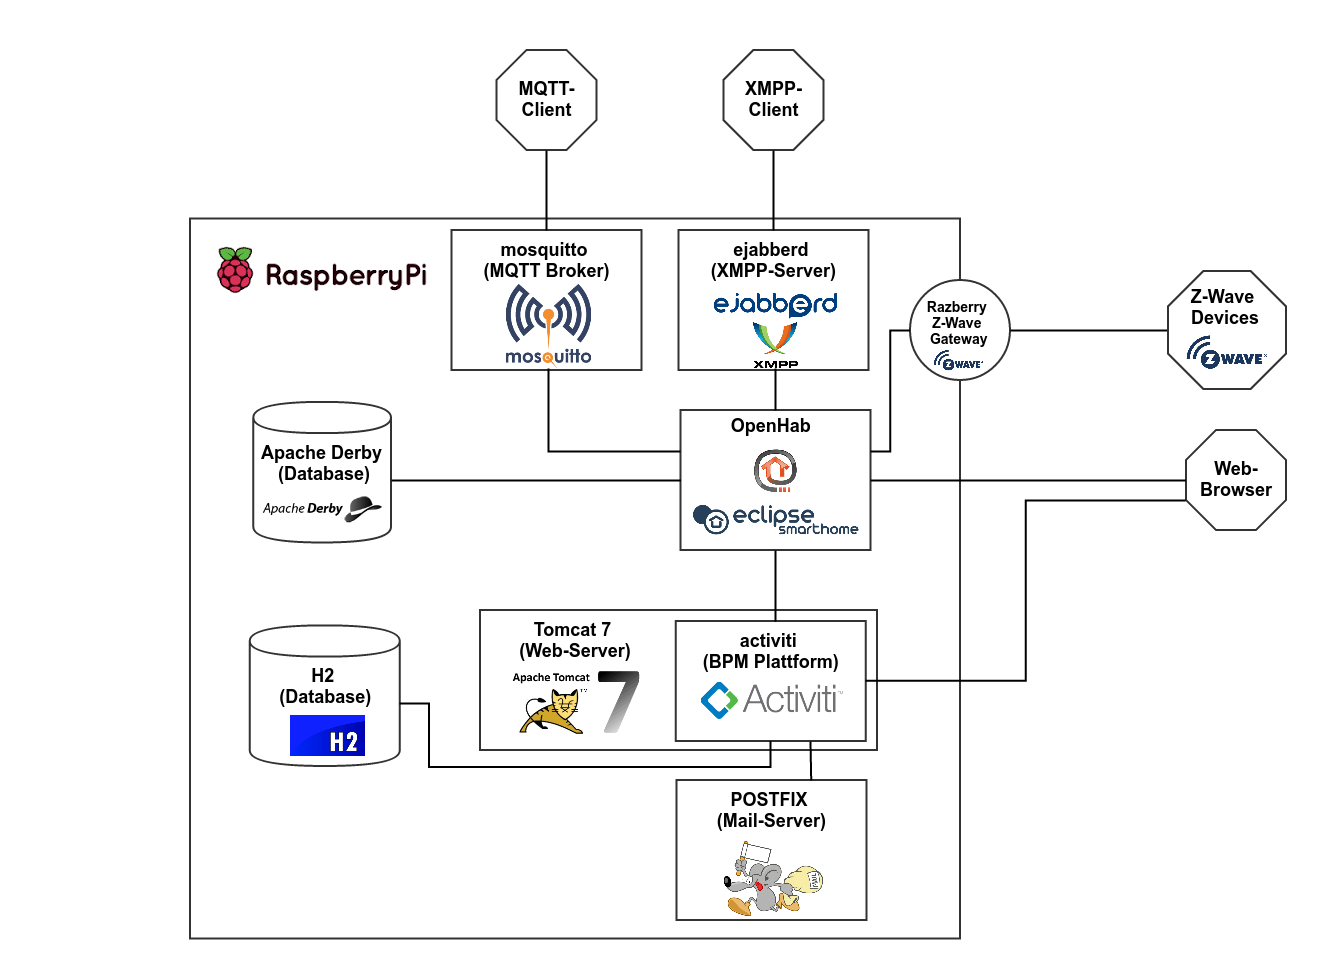
\includegraphics[width=21cm]{./images/Component-Overview}
  \caption{Komponentenübersicht}
\end{figure}
\end{landscape}


\subsection{Prozess / Szenario}
\todo{Finish Process}
Das implementierte Beispiel verwendet nicht alle installierten und konfigurierten Komponenten....
\todo{Beschreibung}
